The first time you boot your HestiaPi, it will go through a setup process which
requires it reboot several times to set everything up.

Follow the on-screen instructions on the LCD when it prompts to connect your
phone to the ``HESTIAPI'' network with HESTIAPI as the password. Once connected
you will automatically be prompted on your phone (or computer) to select your
WiFi network from a list (no hidden SSID supported yet) and enter the password.
If you are not automatically taken you to the wifi setup screen, open
\url{http://192.168.4.1/} in a web browser. This should look similar to what is
in figure \ref{fig:wifi_setup}.

\begin{figure}
  \centering
  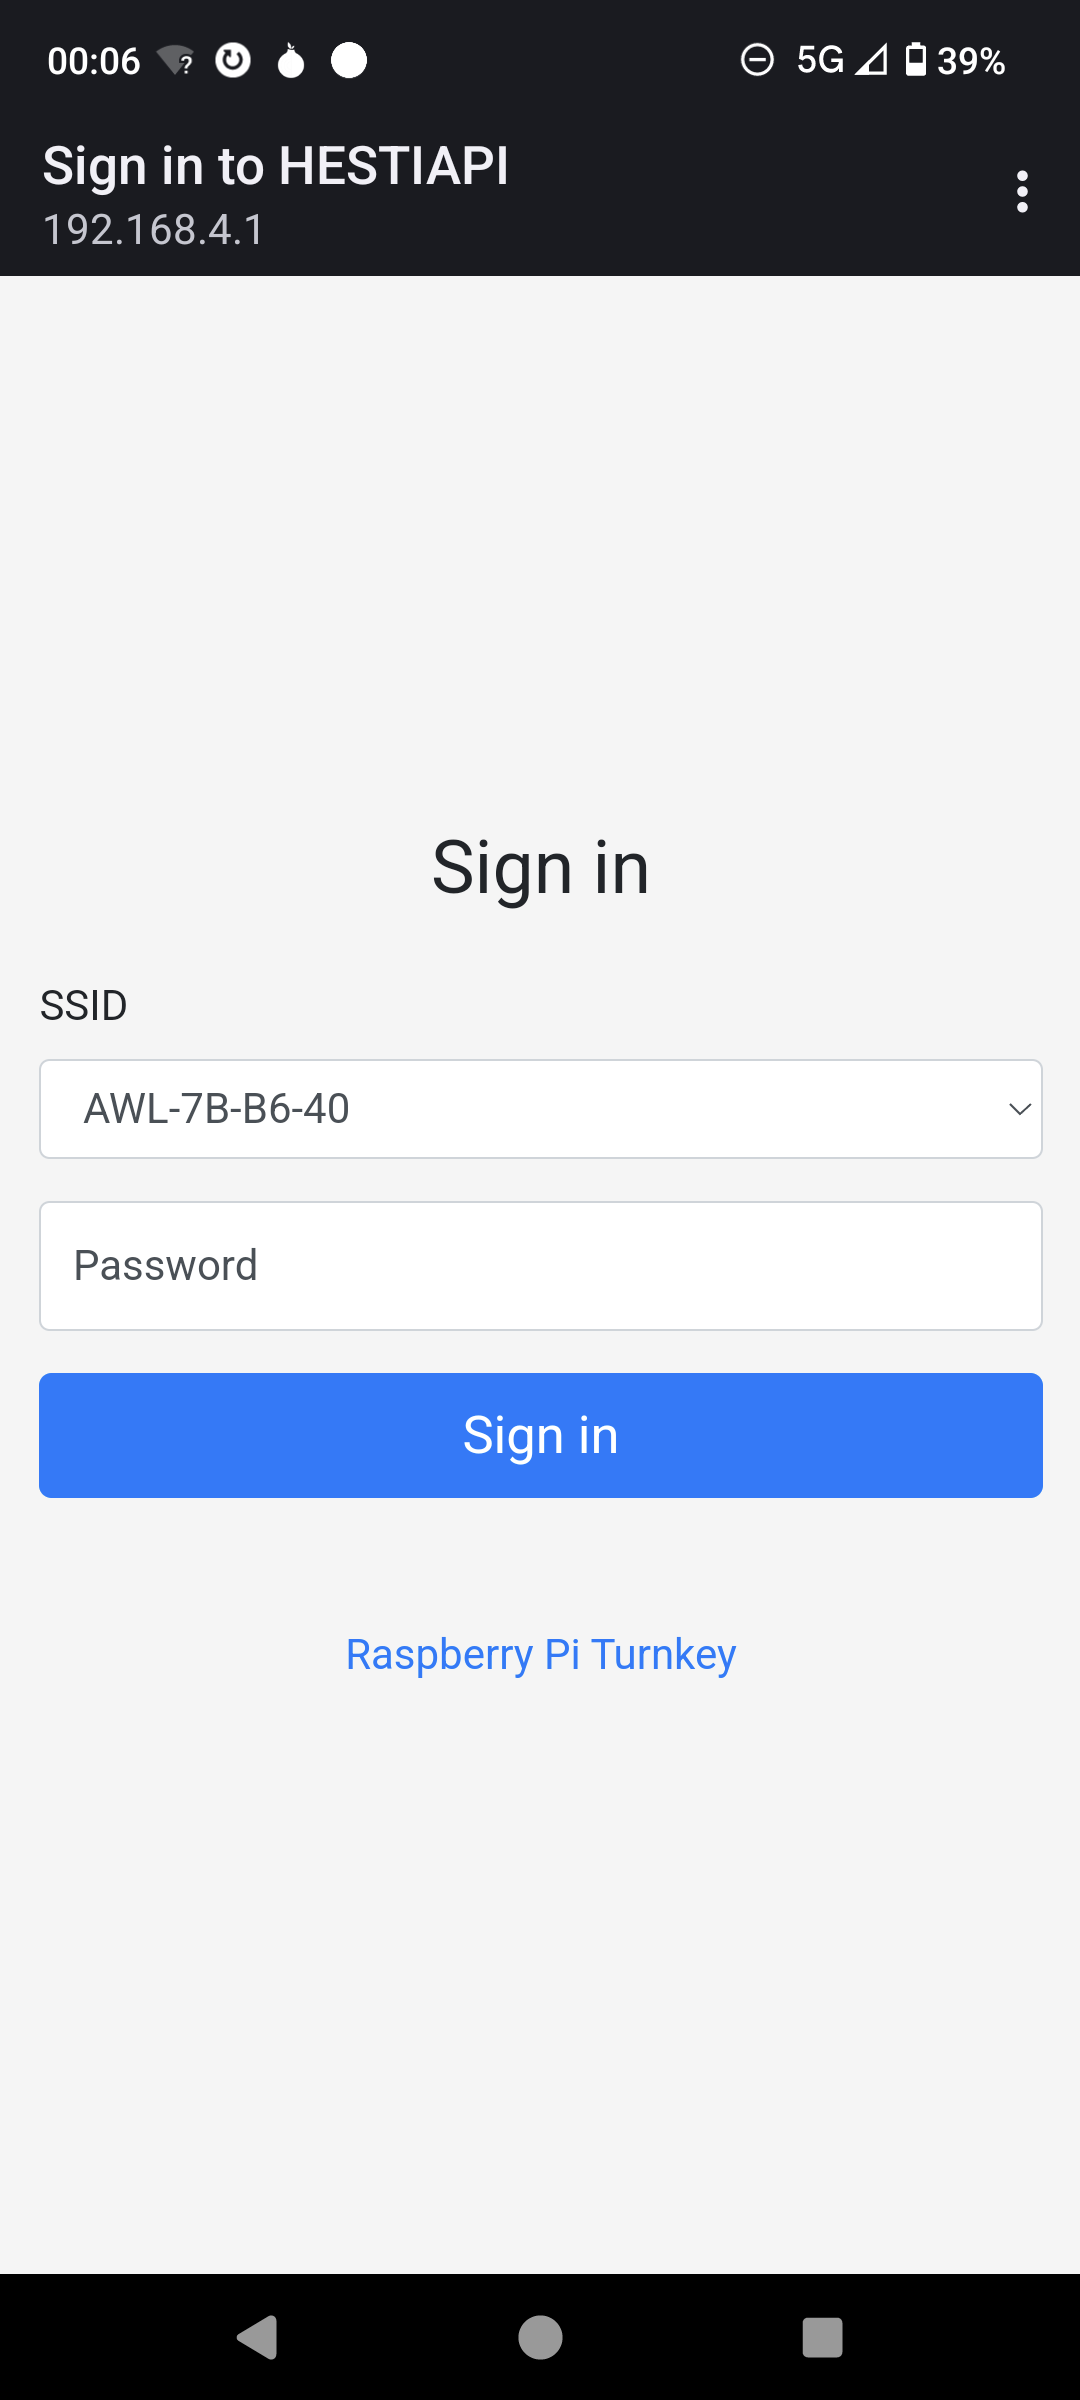
\includegraphics[height=3in]{img/wifi-setup.png}
  \caption{Screen for setting up the HestiaPi's wifi access}
  \label{fig:wifi_setup}
\end{figure}

If you entered the correct wifi info, your HestiaPi will restart and connect to
your network. You should no longer see the HESTIAPI network when you look for
wifi networks on your phone (or computer). The loading screen should show you
the IP address of the HestiaPi while it is booting, and that should be an IP
address from your home network (as opposed to being 192.168.4.1, which is what
it will be if the thermostat is not connected to your wifi network).

When selecting your access point, you will need to choose a 2.4GHz network.
Some routers use both 2.4GHz and 5GHz, however the Rasberry Pi inside of the
HestiaPi does not support 5GHz. This should not be a problem as routers are
configured to be compatible with both, however it's important to know if you
have changed your router settings to disable the 2.4GHz band.

From the time you first turn it on to the time that you are ready to use the
thermostat can take up to 20 minutes. While you are waiting, you may want to
download a mobile app to access the thermostat without having to navigate to
the HestiaPi using a web browser. See section \ref{Mobile App} for more
details.

When the HestiaPi first boots, the LCD UI may start with zeros for the
temperature and humidity. This is normal and the data will update in a minute
or two. If your HestiaPi is using a temperature sensor that does not also have
the ability to sense humidity, the humidity reading will remain as 0\%.

Once the LCD is showing the UI with temperature values, try and load the mobile
app or use your phone or laptop and navigate to:
http://[hestiapi\_IP]:8080/start/index (substituting in your HestiaPi's IP
address where appropriate) and select ``Basic UI''.

You should now be able to control the basic functions from either the app or
your browser.

OpenHAB2 has a great \href{https://community.openhab.org/}{forum} with loads of
information from fellow users who are willing to help you customize your system
to suit your needs.

Please note that the UI of the app, web and LCD may change with software updates
so be sure to back up any customizations you make before running an update.
